\documentclass[14pt]{beamer}

\usetheme[progressbar=frametitle]{metropolis}
\usepackage{appendixnumberbeamer}
\usepackage{caption}
\captionsetup{font=scriptsize,labelfont=small}
\usepackage{booktabs}
\usepackage[scale=2]{ccicons}
\usepackage{graphics,graphicx,epsfig,ulem}
\usepackage{pgfplots}
\usepgfplotslibrary{dateplot}
\usepackage{dblfloatfix}
\usepackage{xspace}
\usepackage{tikz-feynman}
\usetikzlibrary{shapes,snakes}


\newcommand{\themename}{\textbf{\textsc{metropolis}}\xspace}
\usefonttheme[onlymath]{serif}
\title{Strong Coupling Constant Extraction.}
%\subtitle{Georgia Hills, Level 4 project, Supervisor: Dr. D. Ma\^itre}
% \date{\today}
\date{Submitted: \today{}}
\author{Georgia Hills}
\institute{Supervisor: Dr D. Ma\^itre, Level 4 Project, Department of Physics, Durham University}
% \titlegraphic{\hfill\includegraphics[height=1.5cm]{logo.pdf}}


\begin{document}

\maketitle

\begin{frame}{Table of contents}
  \setbeamertemplate{section in toc}[sections numbered]
  \tableofcontents[hideallsubsections]
\end{frame}

\section{Introduction}

\begin{frame}[fragile]{What is ${\alpha_s}$ ?}

The strong force binds quarks and gluons together, and is described by ${\alpha_s}$.
% Is a parameter of Quantum Chromodynamics (QCD) only acts on particles with colour charge, quarks and gluons.  alpha_S tells you how strong that interaction is. The strong force and is responsible for normal matter being stable, 
%i.e the strong force overcomes electromagnetic repulsions and binds quarks and gluons together forming protons, and binds protons and neutrons together to form nucleons. 
%Cannot predict alpha_S so an extraction from experimental data is needed, hence this project, 
\end{frame}

\begin{frame}[fragile]{Data used in the Extraction}
%The data was collected by the Atlas group at Cern, where they measured the cross section of a collision of two protons. Describe the equation. Protons are made of partons namely quarks and gluons. The partons interact not the protons, partons undergo elastic collisions kinetic energy is not conserved. Partons are charged under the strong force they emit lots of collinear radiation which gives rise to jets - groups of hadrons moving in the same direction. We measure the cross section of these jets at root 13 TeV for Z + 2,3,4 jets. and from this data we can extract alpha_s. Will go into more detail later about how this is used etc for the extraction. 
The collision of two protons in the Large Hadron Collider at CERN:
\begin{center}
	${pp \xrightarrow{Z/\gamma}  l^+l^- + X.}$
\end{center}
\begin{figure}
		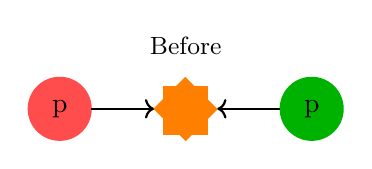
\begin{tikzpicture}[scale=0.8]
			\draw[red!70!white, fill=red!70!white, text=black] (0,0.5) circle (0.5 cm) node{p};
			\draw[green!70!black, fill=green!70!black, text=black] (4,0.5) circle (0.5cm) node{p};
			\draw[->, thick] (0.5,0.5) -- (1.5,0.5);
			\draw[->, thick] (3.5,0.5) --(2.5,0.5);
			\draw[orange, fill=orange] (1.65,0.1) rectangle (2.35,0.85);
			\draw[orange, fill=orange] (2,1)--(1.5,0.5)--(2,0)--(2.5,0.5);
			\draw (2,1.5) node {\small Before};
		\end{tikzpicture}
		\qquad
		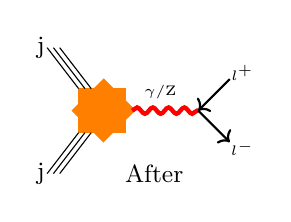
\begin{tikzpicture}[scale=0.8, rotate=270]
			\draw[orange, fill=orange] (1.65,-0.4) rectangle (2.35,0.35);
	     	\draw[orange, fill=orange] (2,0.5)--(1.5,0)--(2,-0.5)--(2.5,0);
	     	\draw[black] (1.65,-0.4)--(1,-0.9);
	     	\draw[black] (1.65,-0.3)--(1,-0.8);
	     	\draw[black] (1.65,-0.2)--(1,-0.7);
	     	\draw[black] (2.35,-0.4)--(3.0,-0.9);
	     	\draw[black] (2.35,-0.3)--(3.0,-0.8);
	     	\draw[black] (2.35,-0.2)--(3.0,-0.7);
	     	\draw[red, ultra thick,decorate,decoration={snake,amplitude=.4mm,segment length=2mm}] (2,0.45)  --(2,1.5);
	     	\draw[<-, thick] (2,1.5)--(1.5,2);
	     	\draw[->, thick] (2,1.5)--(2.5,2);
	     	\draw (3,0.8) node {\small After};
	     	\draw (1,-1) node {\small j};
	     	\draw (3, -1) node {\small j};
	     	\draw (1.7,0.9) node {\tiny $\gamma$/Z};
	     	\draw (2.6,2.2) node {\tiny $l^-$};
	     	\draw (1.4,2.2) node {\tiny $l^+$};

		\end{tikzpicture}

\end{figure}
\end{frame}

\section{Theoretical Context and Motivation}

\begin{frame}[fragile]{Colour Charge, The Quantum Number}
\begin{figure}
	\begin{center}
		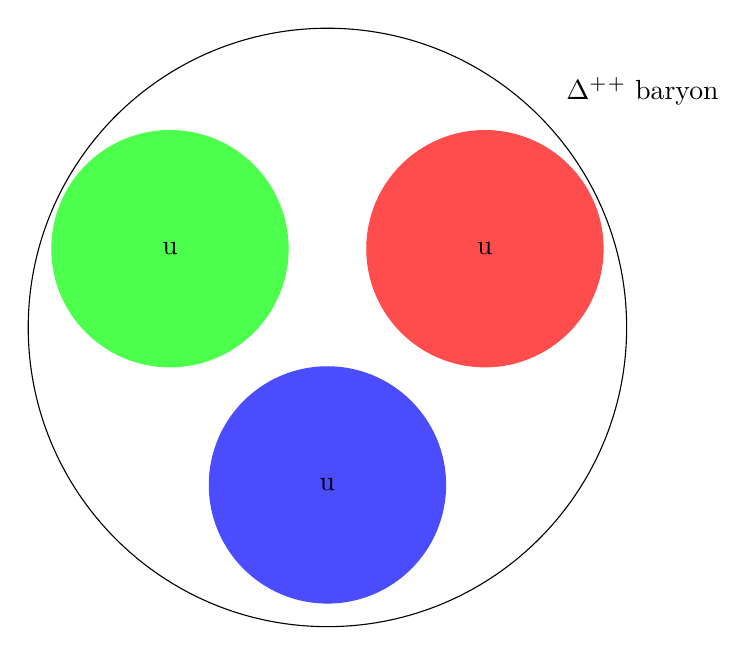
\begin{tikzpicture}
			\draw[red!70!white, fill=red!70!white, text = black] (2,2) circle (1.5 cm) node {u};
			\draw[green!70!white, fill=green!70!white, text=black] (-2,2) circle (1.5 cm) node {u};
			\draw[blue!70!white, fill = blue!70!white, text=black] (0,-1) circle (1.5cm) node {u};
			\draw (0,1) circle (3.8cm);
			\draw (4,4) node { $\Delta$$^+$$^+$ baryon};
		\end{tikzpicture}
	\end{center}
\end{figure}

%QCD is unique as it has an additional quantum number: colour! Baryon has 3 identical fermions, according to Pauli wf needs to be anti-symmetric. But spin, which is 3/2 all up spins totally symmetric under exchange,  parity, all x-> -x, and spatial parts are all symmetric under the exchange of two fermions. so we need another quantum number -> colour charge. This extra quantum number, gives rise to QCD which is different to other aspects of the Standard Model, such as QED so we'll look at QCD in more detail..
\end{frame}

\begin{frame}[fragile]{The Standard Model.}
\begin{figure}
	\begin{center}
		\includegraphics[width=1\textwidth]{STMD.png}
		\caption{Particles of the Standard Model of particle physics (Image: Daniel Dominguez/CERN)}
	\end{center}
\end{figure}


%So for QED the field is mediated by photons similarly for QCD the field is mediated by gluons. However unlike photons which do not carry electromagnetic charge gluons do carry the corresponding charge of the gauge namely colour. This introduces further interactions and complications only seen in QCD.
\end{frame}

%\begin{frame}[fragile]{The QCD Lagrangian}

%{\renewcommand*{\normalfont}{\relax}
%\small
%\begin{equation}  
%\resizebox{0.85\textwidth}{!}
%{ 
%\label{Lag}
%$ \mathcal{L} = \sum_ {q} \overline{\psi}_{q,a} (i\gamma^\mu \partial_\mu \delta_{ab} - g_s \gamma^\mu t_{ab}^C \mathcal{A}_\mu^C  - m_q\delta_{ab})\psi_{q,b} - \frac{1}{4} F_{\mu\nu}^A F^{A \mu\nu}$
%}
%\end{equation}
%}

%The indices a,b run from 1 to the number of colours 3. Mq is the mass of the quarks, q represents the quark flavour of the dirac spinor psi_q,a. First term gives the interaction between a quark and anti-quark. The QCD coupling constant gs is related to as by gs^2/4pi. The tab are the generators of the group there are 8 for the 8 gluons. 
%{\renewcommand*{\normalfont}{\relax}
%\small
%\begin{equation}
%\resizebox{0.85\textwidth}{!}
%{ 
%$F_{\mu\nu}^A  = \partial_\mu \mathcal{A}_\nu^A  - \partial_\nu \mathcal{A}_\mu^A - g_s f^{ABC} \mathcal{A}_\mu^B \mathcal{A}_\nu^C  \qquad [t^A,t^B] = if^{ABC}t^C,$
%}  
%\end{equation} 
%}
%The F describes how the gluon field propagates and is given, these structure constants are like the levi-civita symbol which you have for SU(2). the gs term describes how gluons interact with themselves so for QED you don't have this term. C runs from 1 to 8 as there are 8 gluons. 
%when a quark and gluon interact represented by the second term here, the quarks and gluons colours are rotated in colour space 

%\end{frame}

\begin{frame}[fragile]{Colour Confinement and Asymptotic Freedom}
\begin{figure} 
	\begin{center}
		\includegraphics[width=0.7 \textwidth]{as_allq.jpg}
		\caption{Summary of measurements of ${\alpha_s}$ as a function of ${Q}$ the energy scale. The degree of QCD perturbation theory is given in brackets (NLO: next-to-leading order), etc. This graph was produced by the \textit{Particle Data Group}, see \cite{PPB} }
		\label{allas}
	\end{center}
\end{figure}
%For  example consider rotating a circle in a 2D plane, no matter how far you rotate the circle about the centre you get the same thing. So analogously if we rotate an observable object in colour space it must be colour neutral if we want to preserve this Su3 symmetry. And indeed we find this symmetry to always be preserved and unbroken. IE all observed objects are colour neutral and we never observe quarks or gluons which carry colour charge. this is known as colour confinement. 

%This means if we try separate quarks or gluons inside a colour neutral object their separation is at a measurable scale when the energy of their separation is so large that it greatly overcomes the need to create a new particle. Particles being confined implies that as is large so bonding particles together, seen here. 
%At really high energies quarks and gluons do directly interact, implying as is small here. Asymptotic freedom. 
%So we see that as is not constant and changes with energy so we re-name it the running coupling constant.  
\end{frame}



%\section{Experimental Set-Up at the LHC.}
%\begin{frame}[fragile]{Scattering Process }
% \begin{figure}
%	\minipage{0.4\textwidth}
%		\begin{tikzpicture}[scale=2]
%			\draw[dotted, ->, thick] (0,0) --(0,1.5);
%			\draw[dotted, ->, thick] (-1,0) --(1.5,0);
%			\draw[->, green!30!black, thick] (0,0) --(1,1);
%			\draw[->, black!30!red, thick] (-1,0) --(0,0); 
%			\draw[<-, black!30!red, thick] (0,0) --(1,0);
%			\draw[dotted, <->, thick] (0.5,0.5) arc [start angle= 45, end angle=0, radius = 20pt ];
%			\draw (0.8,0.3) node {$\theta$};
%			\draw[green!30!black] (0.6,0.8) node {\small $p$};
%			\draw[black!30!red] (-0.8, -0.2) node {\small Anti-Proton};
%			\draw[black!30!red] (0.8,-0.2) node {\small Proton};
%			\draw (0,1.7) node {\tiny x-axis};
%			\draw (1.7,0) node {\tiny z-axis};
%			\draw (-0.8,1.5) node {\small a) x-z plane};
%		\end{tikzpicture}
%	\endminipage\hfill
%	\minipage{0.4\textwidth}
%		\begin{tikzpicture}[scale=2]
%			\draw[dotted, ->, thick] (0,0) --(0,1.5);
%			\draw[dotted, ->, thick] (0,0) --(1.5,0);
%			\draw[->, blue, thick] (0,0) --(1,1);
%			\draw[dotted, <->, thick] (0.5,0.5) arc [start angle= 45, end angle=0, radius = 20pt ];
%			\draw (0.8, 0.3) node {$\phi$};
%			\draw[blue] (0.6,0.8) node {\small $p_T$};
%			\draw[black!30!red, fill=black!30!red] (0,0) circle (.2ex);
%			\draw (-0.1,1.7) node {\tiny x-axis};
%			\draw (1.7,0) node {\tiny y-axis};
%			\draw (0.8,1.6) node {\small b) ``Transverse''};
%			\draw (0.8,1.4) node {\small x-y plane};
%			\draw[black!30!red] (0.2, -0.2) node {\small };
%		\end{tikzpicture}
%	\endminipage
%	\caption{a) The scattering centre of two protons, given by the red arrows, with centre of mass scattering angle ${\theta}$ and momentum ${p}$ of the products. b) ${\phi}$ is the azimuthal scattering angle, ${p_T}$ is the transverse momentum which is given by ${p_T = p\sin{\theta}}$ \cite{Sca}.}
%	\label{SCAT}
%\end{figure}
%%%


%Now define the rapidity which is lorentz invariant. We cannot measure the momentum fraction carried by the interacting quarks within the proton and anti-proton, but rapidity is de-coupled from this. So we can define a co-ordinate system using this rapidity, we define the size of the jet R in this co-ordinate space. The cross section is measured for  a given range of momentum and these cross sections are put into bins  like a histogram. 

%\end{frame}


\begin{frame}[fragile]{Cross section vs. ${p_T}$}
	\begin{figure} 
		\begin{center}
			\includegraphics[width=0.7 \textwidth]{xsection_118CT10.png}
			\caption{The Cross section for each number of jets inclusive against the leading jet momentum. The PDF set considered here is CT10nlo for ${\alpha_s = 0.118}$}. %the red bar means the error of the predictions the grey is the experimental error in the cross section. The blue crosses show the ratio of prediction to Data values. Please note that the cross sections have been multiplied by 10-1,2,3 factors for clarity. Note that there is a resonance peak at ~90 GeV coresponding to the mass of the Z boson which is what is expected as we are creating the Z boson which decays into leptons. So this is good it shows that the preedictions are valid. So how do we get the predictions?
			\label{CHI}
		\end{center}
	\end{figure}
	
\end{frame}

\begin{frame}[fragile]{Pros and Cons of multiple jets}
\begin{figure} 
	\begin{center}
		\includegraphics[width=0.7 \textwidth]{2jetvs3jet_totxsection.png}
		\caption{The variation of the error of cross section covered for a given range of ${\alpha_s}$. A higher number of jets corresponds to a larger cross sectiin considered hence a lower error on that cross section measurement. The PDF used was MSTW08cl for the central scale. }
		\label{2jetvs3jet
		}
	\end{center}
\end{figure}

%benefits of using multiple jets. 
\end{frame}

\begin{frame}[fragile]{FastNLO}
	\begin{itemize}
		\item We need to compare experimental data with theoretical predictions in order to extract ${\alpha_s}$. 
		\item Calculating theoretical predictions is time consuming.
		
	\end{itemize}
	%The point of Fastnlo is to speed up the calculating predictions process. So we want to calculate the nearly the same cross section many times, more runs = lower statistical error. Just to note that the perturbative predictions of these observables depend on a_s so thats how we can use predicitons to find a_s. So how to simplify this?
	%approximate the integrals into a sum allows us to separate the cin which are coefficients, and the PDF and alpha bit, Pdfs are given by the f where x is the fraction of the total hadron momentum carried by the parton. So fastnlo calculates the c's and stores them in a table for easy reading later. The mu_R and mu_F are scales and the ci are dependent on these scales so the ci's are stored in flexible -scale tables. 
	
	{\renewcommand*{\normalfont}{\relax}
		\small
		\begin{center}
			\resizebox{0.85\textwidth}{!}
			{ 	
				${\sigma(\mu_R \ \mu_F) = \sum_{i,n} \int_{0}^{1}  dx_1 \ \alpha_s(\mu_R) c_{i,n} \left( \frac{x_{Bj}}{x}, \mu_R, \mu_F \right) f_i(x, \mu_F)}$,
			}
		\end{center}
	}	
\end{frame}	

\begin{frame}[fragile]{Factorisation and Renormalisation scales}
	%The matrix element gives the amplitude for a given process and divergences appear due to two sources:
	\begin{itemize}
		\item ${\mu_R}$: Ultra-Violet Divergences - appear due to large momenta loops. %in the feynman diagrams which represent the amplitude of a prcoess. Divergences occur when the energy of the interaction becomes arbitratirly large. Here alphas is small at large energy so can be treated perturbatively. 
		\item ${\mu_F}$: Infrared Divergences - appear due to i) a virtual or real particles reaching zero momentum ii) a massless particle radiates another massless particle. %like a gluon radiating collinear gluons. Occur at small energies when alpha s is large so non-perturbative. Essentially determines the point between when perturbation theory is valid and when it isn't. 
		
	\end{itemize}
	
	These both lead to ${\alpha_s}$ depending on these unphysical scales, hence observables should not depend on them. %however in practice observables do due to approximations. So I calculate predications at varying scales in order to ascertain the error introduced by this arbitrary scale neccessary for calculating things.
	
\end{frame}

\section{PDF's}


\begin{frame}[fragile]{What are PDF's?}
	
	PDF's are number density functions associated with finding certain partons inside the proton. 
	%pdfs depend on the fraction of the protons momentum the quark is carrying. can't be predicted and we fit them to experimental data. however there are physical constraint such as the quantum numbers should be conserved charge conserved and momentum conserved. ie when you add the fractions times the parts together you should get the total picture ie the proton. 
	
\end{frame}

\begin{frame}[fragile]{How PDF's are generated}
	\begin{figure}
		\begin{center}
			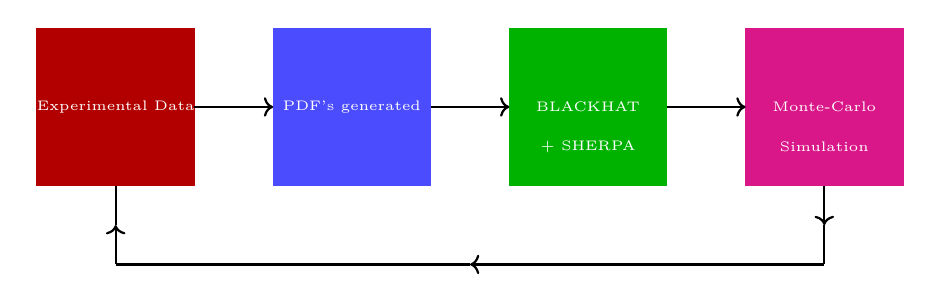
\begin{tikzpicture}
			\draw[red!70!black, fill = red!70!black, text=white] (0,0) rectangle (2,2) node[pos=0.5] {\tiny Experimental Data};
			\draw[blue!70!white, fill=blue!70!white, text=white] (3,0) rectangle (5,2) node[pos=0.5] {\tiny PDF's generated};
			\draw[green!70!black, fill=green!70!black, text=white] (6,0) rectangle (8,2) node[pos=0.5] {\tiny BLACKHAT};
			\draw[white](7,0.5) node {\tiny + SHERPA};
			\draw[magenta!90!black, fill=magenta!90!black, text=white] (9,0) rectangle (11,2);
			\draw[white] (10,1) node {\tiny Monte-Carlo};
			\draw[white] (10,0.5) node {\tiny Simulation};
			\draw[->, black, thick] (2,1) --(3,1);
			\draw[->, black, thick] (5,1) --(6,1);
			\draw[->, black, thick] (8,1) --(9,1);
			\draw[->,black,thick] (10,0) -- (10,-0.5);
			\draw[-,black,thick] (10,-0.5) -- (10,-1);
			\draw[->,black,thick] (10,-1) -- (5.5,-1);
			\draw[-,black, thick] (5.5,-1) --(1,-1);
			\draw[->,black,thick] (1,-1) -- (1,-0.5);
			\draw[-, black, thick] (1,-0.5) --(1,0);
			
			\end{tikzpicture}
		\end{center}
	\end{figure}
	%phase space_ a phase space is a space in which all possible states of a system are represented, with each possible state corresponding to one unique point in the phase space
\end{frame}


\section{Statistical Analysis and Extraction Procedure}
\begin{frame}[fragile]{Extraction Procedure}


{\renewcommand*{\normalfont}{\relax}
\small
\begin{center}
\resizebox{0.85\textwidth}{!}
{ 
$\chi^2(\alpha_s(M_z)) = (\bold{y_t}(\alpha_s(M_z))-\bold{y_d})^T\hat{C^{-1}}(\bold{y_t}(\alpha_s(M_z))-\bold{y_d} )\ \ $
}  
\end{center} 
}

{\renewcommand*{\normalfont}{\relax}
\small
\begin{center}
\resizebox{0.5\textwidth}{!}
{ 
$C = C_{exp} + C_{PDF} + C_{theory} \ \ $
}  
\end{center} 
}
%The Chi squared function must be minimised, the minima's position corresponds to the best value of alpha_S. Chi squared shows a goodness of fit bit the experimental data yd and the predictions yt. C is the covariance matrix measures how the change of one variable is associated with another. So if two variables are completely independent their covariance matrix is a 2x2 diagonal whose elements are the errors of the variables squared. so n variables has an nxn matrix. each element has dimensions error squared. 

%In this case the covariance matrix has three parts.
\end{frame}

\begin{frame}[fragile]{The Covariance Matrix}

Consider two variables a and b with errors 2 and 3 respectively. Their covariance matrices are:
	\begin{minipage}{.5\linewidth}
		\centering
		\[(A)\left[\begin{array}{cc}
		4 & 0 \\
		0 & 9
		\end{array}\right]\]
		Independant Variables
	\end{minipage}%
	\begin{minipage}{.5\linewidth}
		\centering
		\[(B)\left[\begin{array}{cc}
		4 & 6 \\
		6 & 9
		\end{array}\right]\]
		Dependent Variables
	\end{minipage}

\end{frame}
\begin{frame}[fragile]{Calculating ${C_{exp}}$}
There are three sources of experimental error: \begin{itemize}
	\item Statistical
	\item Systematic
	\item Luminosity
\end{itemize}
%Stat- fundamental to each measurement and is uncorrelated. Cstat is diagonal and is statistical errors squared.
%Luminosity- how many particles in a given xsection in a given time, has the dimensions of flux. higher luminosity- more likely we get collisions, more likely the process we're interested in actually happens. There is an uncertainty with this which is fixed at 2.1% 
%Systematic error occurs due to imprecision of instruments and is pretty much fixed. 

\end{frame}

\begin{frame}[fragile]{The sturcture of the Covariance matrix}

\begin{figure} 
	\begin{center}
		\includegraphics[width=0.7 \textwidth]{colourplot_C_full.png}
		\caption{A colour plot showing the structure of the covariance matrix, note that the bottom right corner corresponds to 2 jet electron channel. }
		\label{Cfull
		}
	\end{center}
\end{figure}
\end{frame}
	
	






\section{Conclusion}

\begin{frame}[fragile]{Conclusions}
	

\begin{figure} 
	\begin{center}
		\includegraphics[width=0.7 \textwidth]{CT10nlo0_curvefit.pdf}
		\caption{A ${\chi ^2}$ test for the CT10nlo PDF at all scale combinations considered. The blue squares represent the minima of each curve and the scale error is found by the envelope of statistics method.}
		\label{CHI}
	\end{center}
\end{figure}

%We now take all that together C_pdf, Cexp and C theory to minimise Chi and find the best value of alpha_s. there are still some corrections to consider, for example correspondance between parton and hadron level and factorisation and renormalisation which is what needs to be done to improve on this. 
\end{frame}

{\setbeamercolor{palette primary}{fg=black, bg=yellow}
\begin{frame}[standout]
  Questions?
\end{frame}
}

\appendix


\begin{frame}[allowframebreaks]{References}

\begin{thebibliography}{99}
\bibitem{BOOK} M. Peskin and D. Schoeder, (2005), \textit{An Introduction to Quantum Field Theory.}
\bibitem{PPB} Particle Date Group, (2017), \url{http://pdg.lbl.gov/2018/reviews/rpp2018-rev-qcd.pdf}, \textit{ Review of Particle Physics: 9. Quantum Chromodynamics}
\bibitem{DMP}M. Johnson and D. Maitre, (2018), \url{https://arxiv.org/pdf/1711.01408.pdf}, \textit{Strong coupling constant extraction from high-multiplicity Z ${^+}$ jets observables.}
\bibitem{CPDF} S. Alekhin, J. Blumein, and S. Moch, (2012), \url{https://arxiv.org/pdf/1202.2281.pdf}, \textit{Parton distribution functions and benchmark cross sections at NNLO, pg 44.} 

\end{thebibliography} 

\end{frame}
\begin{frame}[fragile]{The Structure of PDF's}
	\begin{figure}
		\begin{center}
			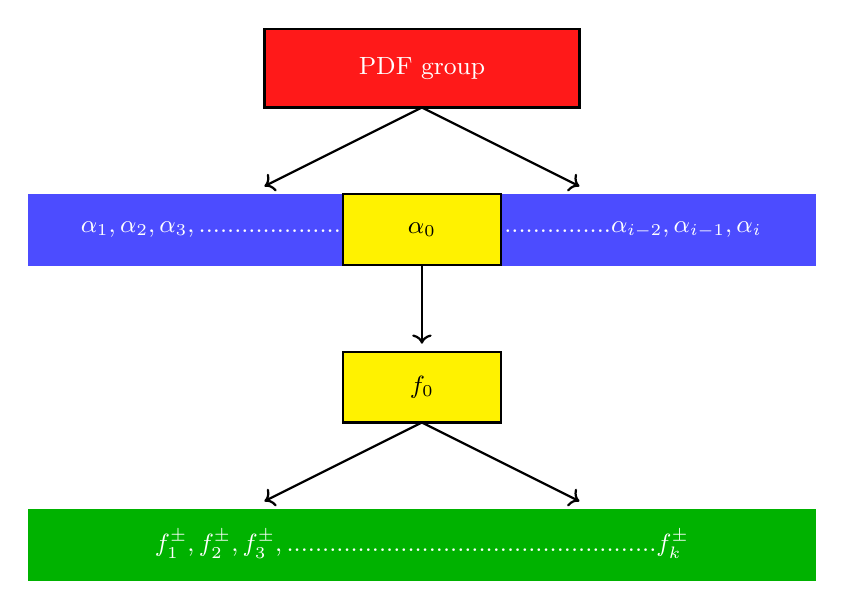
\begin{tikzpicture}
			\draw[black, thick, fill = red!90!white, text=white] (-2,-1) rectangle (2,0) node[pos=0.5] {\small PDF group};
			\draw[->, black, thick] (0,-1) -- (-2,-2);
			\draw[->, black, thick] (0,-1) -- (2,-2);
			\draw[blue!70!white, fill=blue!70!white, text=white] (-5,-3) rectangle (0,-2.1) node[pos=0.5] {\small $\alpha_1, \alpha_2, \alpha_3,........................$ };
			\draw[blue!70!white, fill=blue!70!white, text=white] (0,-3) rectangle (5,-2.1) node[pos=0.5] {\small .$.................. \alpha_{i-2}, \alpha_{i-1}, \alpha_i$ };
			\draw[black, thick, fill=yellow, text=black] (-1,-3) rectangle (1,-2.1) node[pos=0.5] {\small $\alpha_0$};
			\draw[->, black, thick] (0,-3) -- (0,-4);
			\draw[black, thick, fill=yellow, text=black] (-1,-5) rectangle (1,-4.1) node[pos=0.5] {\small $f_0$};
			\draw[->, black, thick] (0,-5) -- (-2,-6);
			\draw[->, black, thick] (0,-5) -- (2,-6);
			\draw[green!70!black, fill = green!70!black, text=white] (-5,-7) rectangle (5,-6.1) node[pos=0.5] {\small $f_1^\pm, f_2^\pm, f_3^\pm,....................................................f_k^\pm$};
			
			\end{tikzpicture}
		\end{center}
	\end{figure}
	
	%The PDF's are key to finding a_S, Each PDF is generated for a particular value of a_S. So we take the pdf's and run them through fastnlo which is sort of like a mini monte carlo simulation and it spits out the cross sections for 2,3,4 jets. gives the theoretical values of the cross section. then use these xsections for each pdf at each a_s to find Cpdf, there are 2 types of pdf used here. 
	% NN two NN pdf's contain replicas all equally valid so there are N pdf's for each pdf so find the average and standard deviation then use this equation errorxerror to find the Cpdf
	% the other type is more complicated. Firstly they are parameterised by K parameters which can be varied. Fo these psd's there is a central valus of a_S, alpha_0 which we treat separately to the other values of a_S. For this a_0 a x^2 test is peformed not by me, when it is minimized this corresponds to the best fitting pDF with the best parameters. 
	
	
\end{frame}

\begin{frame}[fragile]{Calculating ${C_{PDF}}$}
	%SO how do we calculate CPDF in this case? We use the other PDF's in this set with slightly different parameters. tHEY ARE obtained by considering the 1sigma variation on the best value. They come in pairs f^k+_ tand you get an asymmetric error. the asymmetric error for each bin is calculated using. here sigma represents the cross sections calculated for the fk pairs. so we average these two then convert to a matrix using equation before 
	
	
	{\renewcommand*{\normalfont}{\relax}
		\small
		\begin{equation}
		\resizebox{0.8\textwidth}{!}
		{ 
			$\Delta\sigma^+_{PDF} = \sqrt{\sum_{k=1,n_{PDF}} {\max(0, +\sigma_{k,+} - \sigma_0, +\sigma_{k,-} -\sigma_0)^2}} \     \ \cite{CPDF}$
		}  
		\end{equation} 
	}
	
	{\renewcommand*{\normalfont}{\relax}
		\small
		\begin{equation}
		\resizebox{0.8\textwidth}{!}
		{ 
			$\Delta\sigma^-_{PDF} = \sqrt{\sum_{k=1,n_{PDF}} {\min(0, -\sigma_{k,+} + \sigma_0, -\sigma_{k,-} +\sigma_0)^2}} \    \  \cite{CPDF}$
		}  
		\end{equation} 
	}
	
\end{frame}

\begin{frame}[fragile]{Calculating ${C_{PDF}}$ for general ${\alpha_s}$}
	%the other values of c_PDF' are described by one PDF withe the central best fit parameters f0. we use Cpdf(a0), its converted to a percentage error matrix using:  
	
	\begin{equation} \label{PERREV} C_{\%} = \dfrac{C_{PDF}^{i,j}(\alpha_0) \times 100}{ \sigma_{0}^{i} \times  \sigma_{0}^{j}}, \end{equation} 
	
	%then use C% to find cpdf for the other as values, we use this equation in reverse but now these cross sections are the cross sections generated from the PDF's at these other non central alpha_S values. 
	
\end{frame}

\end{document}